\documentclass{beamer}
\usepackage[utf8]{inputenc}
\usepackage{xeCJK} 
\usepackage[T1]{fontenc}
\usepackage{mathabx}
\usepackage{amsmath} 
\usepackage{mathpazo}
\usepackage{bibentry}
\usepackage{tikz}
\usepackage{caption}
\usepackage{graphicx}
\usepackage{subfigure}
\usepackage{animate}

\usetikzlibrary{scopes}
\def\iangle{35} % Angle of the inclined plane
\def\down{-90}
\def\arcr{0.5cm} % Radius of the arc used to indicate angles

\usetheme{Boadilla}
\usecolortheme{wolverine}
\useoutertheme{miniframes}

\title{VP160 Recitation Class VI}
% \subtitle{Non-inertial FoR}
\author{Zeyi Ren}
\institute{UM-SJTU Joint Institute}

\begin{document}

\maketitle

\frame{\tableofcontents}
\section{Lagrangian Mechanics}
\begin{frame}
  \begin{block}{Generalized coordinates}
    Any coordinates describing motions.
  \end{block}\pause
  e.g.
  \begin{figure}[H]
  \centering
  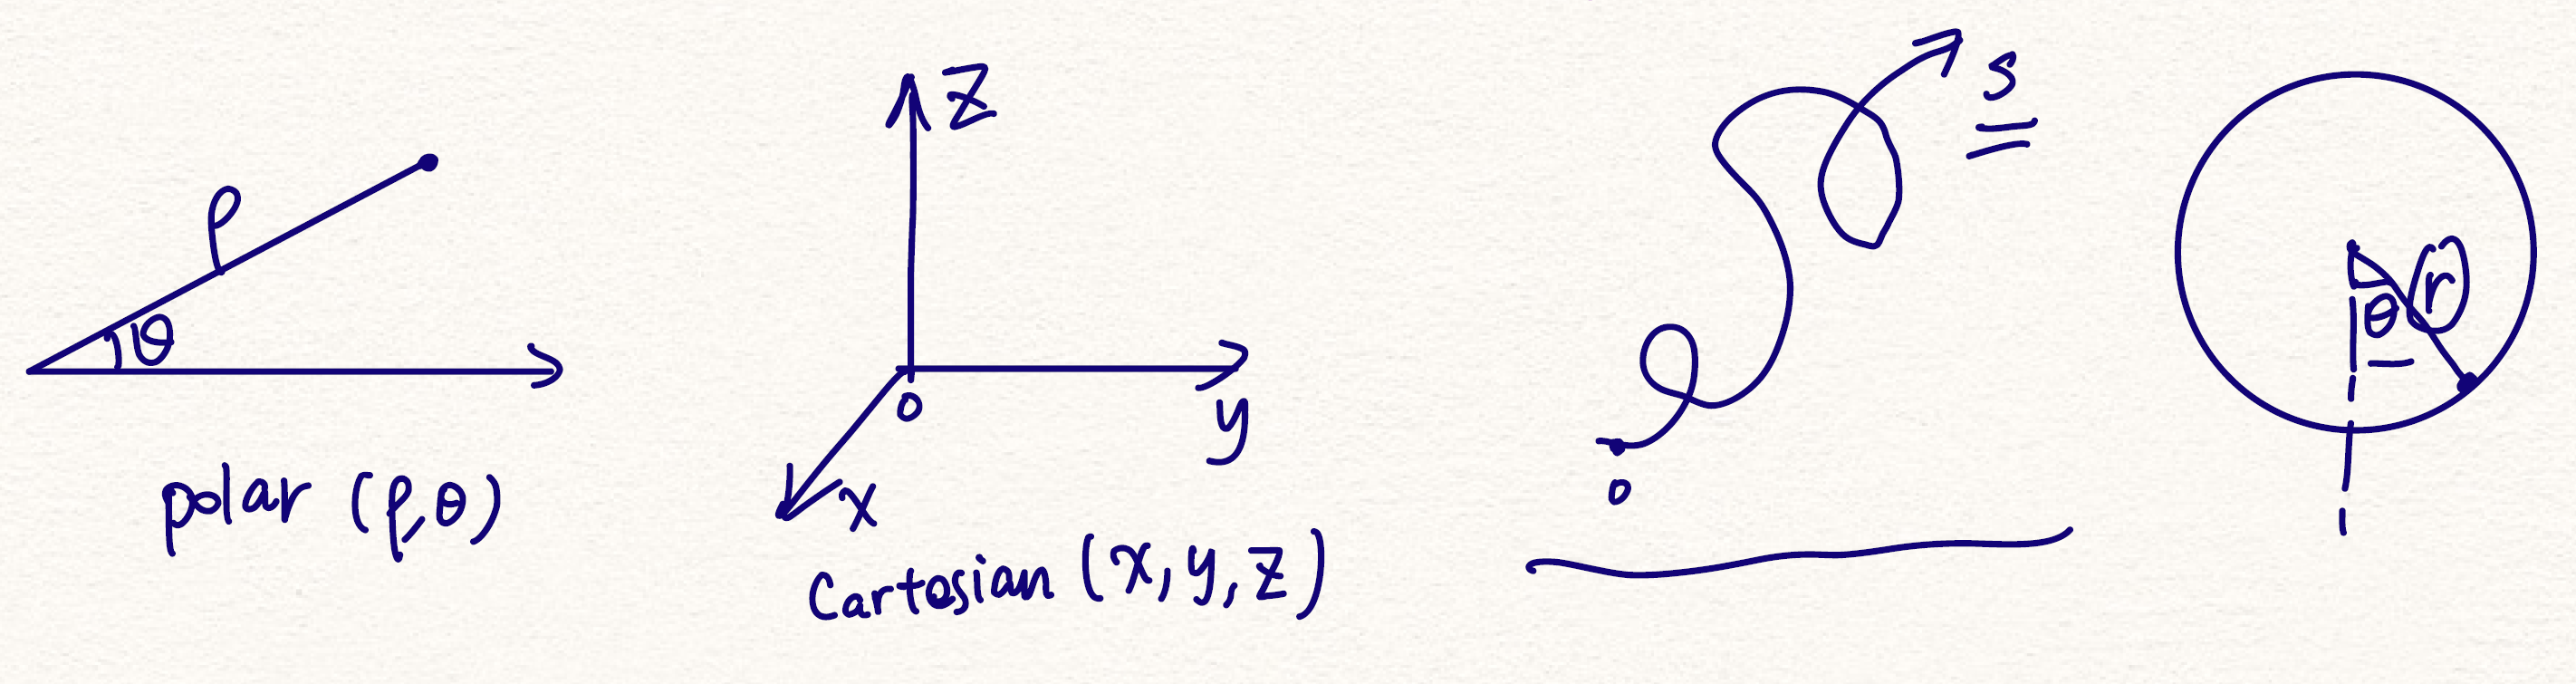
\includegraphics[width= 0.8\linewidth, angle =0]{example1.png}
  % \caption{.}
  \label{fig:1}
  \end{figure}\pause
  $$
    \left\{\begin{array}{l}
      q_1(t)\\
      q_2(t)\\
      ...\\
      q_n(t)
      \end{array}\right.\Rightarrow 
      \left\{\begin{array}{l}
        \dot{q_1(t)}\\
        \dot{q_2(t)}\\
        ...\\
        \dot{q_n(t)}
      \end{array}\right. \text{(generalized velocity)}
  $$
\end{frame}

\begin{frame}
  \begin{block}{Degree of freedom (usually denoted by $f$)}
    The minimum number of independent generalized coordinates needed to describe the system's motions.
  \end{block}\pause
  In general, 
  $$
  f = 3N - m
  $$
  where $N$ is the number of particles, and $m$ is the number of constraints (number of equations that relate unknowns).\pause\\
~\\
 \textcolor{blue}{Exercise 1}\\
 Find the degree of freedom:
 \begin{figure}[H]%
  \centering
  \subfigure[]{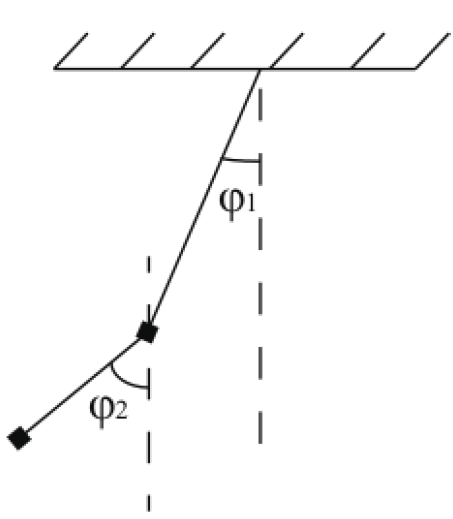
\includegraphics[width=0.12 \linewidth, angle =0]{ex11.png}}
  \label{11}
  \subfigure[]{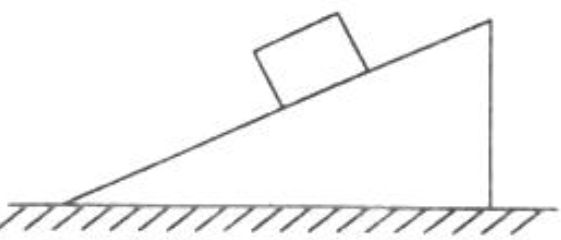
\includegraphics[width=0.12 \linewidth, angle =0]{ex12.png}}
  \label{12}
  % \caption{Step Response}
\end{figure}
\end{frame}

\begin{frame}
  \begin{block}{Hamilton's Principle}
    \begin{center}
    Real path $\Longleftrightarrow$ $\delta S = 0$\\ ($\delta$: variational differential, $S$ is a functional: a function that maps functions into numbers.)
    \end{center}
  \end{block} \pause
  $$\Downarrow \text{How?}$$
  \begin{block}{Euler-Lagrange Equation}
    For $i = 1, 2,...,f$:
    $$
    \frac{d}{dt}(\frac{\partial L}{\partial \dot{q_i}})-\frac{\partial L}{\partial q_i} = 0
    $$
  \end{block}\pause
  Learn more about variational and how to derive Hamilton's Principle, visit\\ \url{https://zhuanlan.zhihu.com/p/126115834}\\ \url{https://zhuanlan.zhihu.com/p/139018146}
\end{frame}

\begin{frame}
\textcolor{blue}{Exercise 2}

A simple pendulum of length $b$ and mass $m$ moves attached to a massless rim of radius $a$ rotating with
constant angular velocity $\omega$. How many degrees of freedom do we have here? Find the Lagrangian.
\begin{figure}[htbp]
\centering
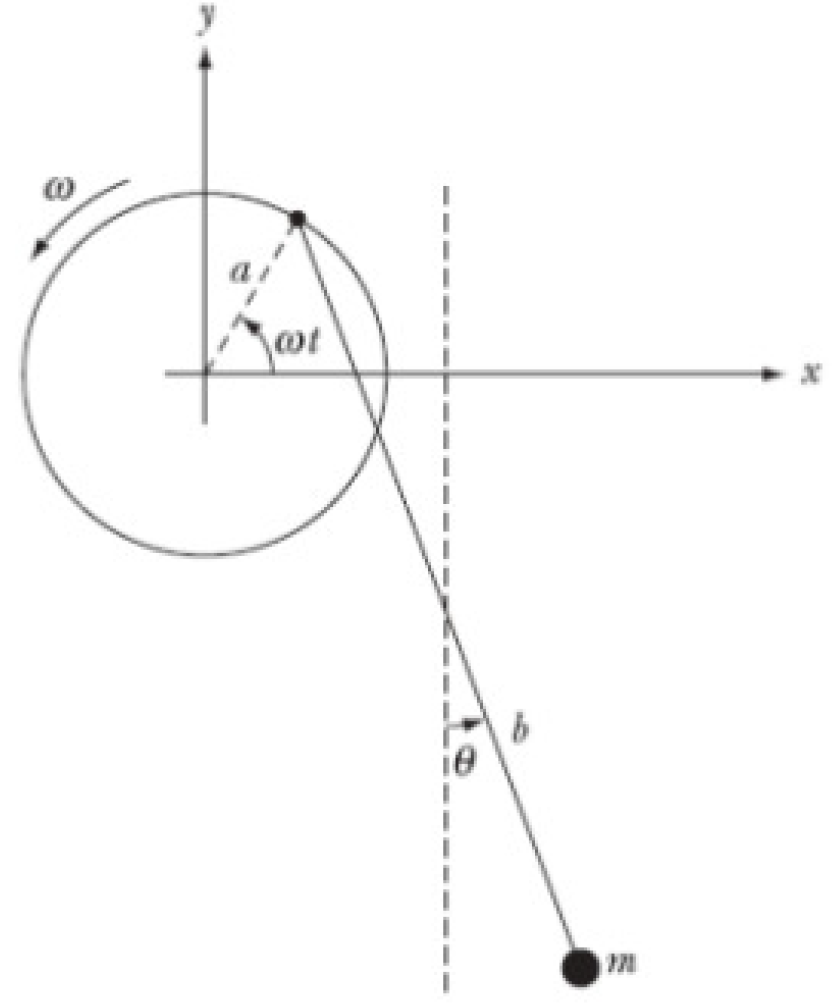
\includegraphics[width=0.4 \linewidth, angle =0]{ex2.png}
% \caption{.}
\label{fig:2}
\end{figure}
\end{frame}

\begin{frame}
\textcolor{blue}{Exercise 3}

Find the equations of motion of a particle of mass $m$ constrained to move on the surface of a sphere, acted upon a conservative force $\mathbf{F}=F_0\hat{n_\theta}$ with $F_0$ a constant.\\\
~\\
Hint. To find the potential energy find the scalar product $\mathbf{F}\cdot d\mathbf{r}$ for the infinitesimal displacement on the sphere and use the fact that it is equal to $-dU$ (the force is conservative).
\end{frame}
\begin{frame}
\textcolor{blue}{Exercise 4}

Double pendulum:\\
(1) identify the generalized coordinates;\\
(2) find the Lagrangian;\\ 
(3) write down the Euler-Lagrange equations of motion;
\begin{center}
  \animategraphics[width=5cm,height=5cm, autoplay, loop]{10}{demo-}{0}{499}
\end{center}
\end{frame}

\section{Momentum}
\begin{frame}
  \begin{block}{Definition}
    $$\vec{p} = m\vec{v}$$
  \end{block}\pause
  \begin{block}{Rewrite Newton's second law}
    $$\vec{F}=\frac{d\vec{p}}{dt}$$ (when $m$ is not varying, $F = m\frac{d\vec{v}}{dt}=m\vec{a}$)
  \end{block}\pause
  \begin{block}{Impulse Theorem}
    $$\vec{p_2}-\vec{p_1}=\int_{t_1}^{t_2}\vec{F}dt$$
  \end{block}\pause
  \begin{itemize}
    \item If $\vec{F_{ext}} = 0$, for a system, $\Delta\vec{p} = 0 \Leftrightarrow p = \text{Const}$ (Conservation of momentum)
  \end{itemize}
\end{frame}

\section{Collision}
\begin{frame}{Application of Conservative of Momentum}
  \begin{itemize}
    \item Non-central Collision (e.g. explosion)
    $$\vec{p_{before}} = \vec{p_{after}}$$\pause
    \item Central Collision
    \begin{itemize}
      \item Elastic
      \begin{itemize}
        \item $e = (\vec{v_2}'-\vec{v_1}')/(\vec{v_1}-\vec{v_2})= 1$
        \item Conservation of energy
      \end{itemize}\pause
      \item Inelastic
      \begin{itemize}
        \item $e < 1$
        \item Energy loss
      \end{itemize}\pause
      \item Completely Inelastic
      \begin{itemize}
        \item $e = 0$
        \item stick to each other
      \end{itemize}
    \end{itemize}
  \end{itemize}
\end{frame}

\begin{frame}
\textcolor{blue}{Exercise 5}

Assume $m_1$, $m_2$, $m_3$, $k$ is known. Release $m_1$, the collision between $m_1$ and $m_2$ is completely inelastic. Find $h$ so that $m_3$
can just leave the ground.
\begin{figure}[htbp]
\centering
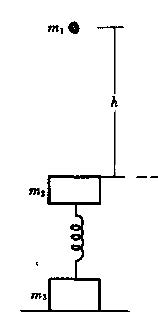
\includegraphics[width=0.2 \linewidth, angle =0]{ex5.png}
% \caption{.}
\label{fig:5}
\end{figure}

\end{frame}

\section{Center of Mass}
\begin{frame}
  \begin{block}{Center of Mass}
    $$r_C = \frac{\sum m_ir_i}{\sum m_i}$$ 
    $$ r_C = \frac{\int_{}^{} r_i dm}{\int_{}^{} dm}$$
  \end{block}\pause
  \begin{block}{Pappus Law}
    First Theorem: $$S = 2\pi sx$$
    Second Theorem: $$V = 2\pi Ax$$
  \end{block}
  where $x$ is the distance from the reference axis and the center of mass.
  
\end{frame}

\begin{frame}
  \begin{figure}[H]
    \centering
    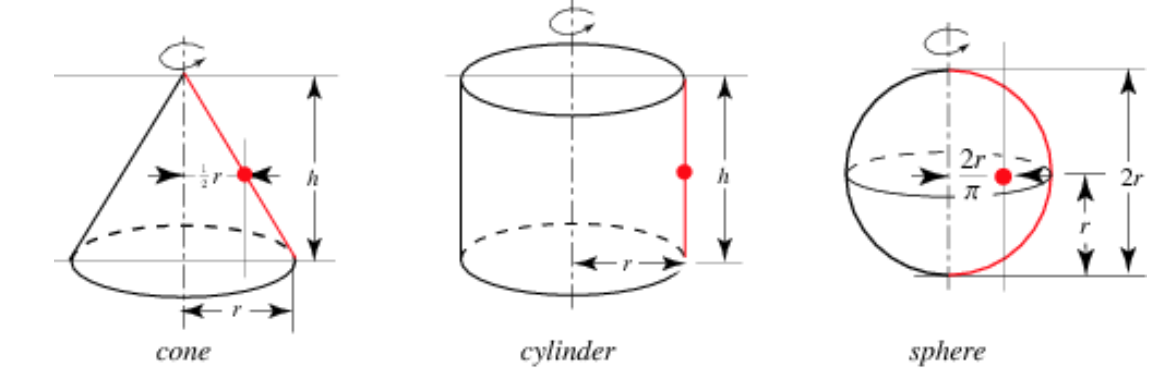
\includegraphics[width=0.6 \linewidth, angle =0]{example3.png}
    % \caption{.}
    \label{fig:6}
    \end{figure}
    \begin{figure}[htbp]
    \centering
    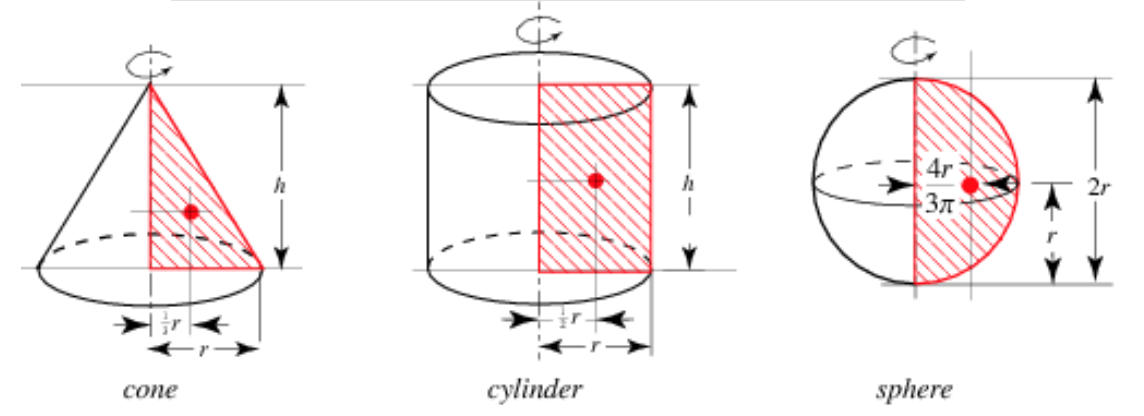
\includegraphics[width=0.6 \linewidth, angle =0]{example2.png}
    % \caption{.}
    \label{fig:7}
    \end{figure}\pause
    \begin{itemize}
      \item An important fact: $$\vec{F_{ext}} = 0 \Leftrightarrow \vec{p} = Const \Leftrightarrow \vec{v_c} = Const$$
    \end{itemize}
\end{frame}

\section{Rocket Propulsion}
\begin{frame}
  \begin{block}{Rocket Propulsion}
    $$mv + Fdt = (m+dm)(v+dv)-udm$$
    $$m\frac{dv}{dt} = (u-v)\frac{dm}{dt}+ F$$
    \end{block}
    \textcolor{blue}{Reminder}\\
    What FoR are we looking at?
\end{frame}

\begin{frame}
\textcolor{blue}{Exercise 6}

A rope with length $l$ and mass $m$ is placed vertically. At the beginning, the lower end of the rope just touches the ground. Release the rope, find the support force of the ground with respect to $x$.
\begin{figure}[htbp]
\centering
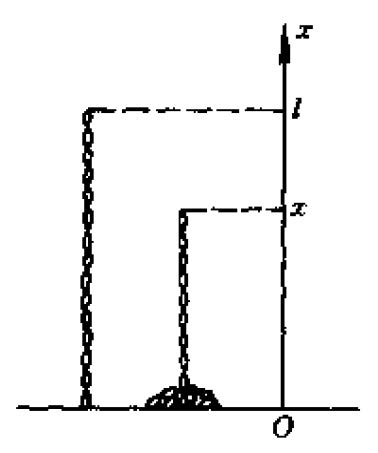
\includegraphics[width=0.4 \linewidth, angle =0]{ex6.png}
% \caption{.}
\label{fig:6}
\end{figure}

\end{frame}


\begin{frame}{Reference}
  \begin{thebibliography}{9}
  \setbeamertemplate{bibliography item}[article]
  \bibitem{C} Yigao Fang.\\
  \textcolor{black}{VP160 Recitation Slides.}\\
  2020
  \bibitem{C} Haoyang Zhang.\\
  \textcolor{black}{VP160 Recitation Slides.}\\
  2020
  % \setbeamertemplate{bibliography item}[book]
  % \bibitem{C} Yousheng Shu (舒幼生).\\
  % \textcolor{black}{\textit{Mechanics (力学)}}\\
  % Peking University Press, 2005
  % \setbeamertemplate{bibliography item}[book]
  % \bibitem{C} Jiafu Cheng (程稼夫).\\
  % \textcolor{black}{\textit{中学奥林匹克竞赛物理教程:力学篇}}\\
  % University of Science and Technology Press, 2013
  \end{thebibliography}
  \end{frame}
  \end{document}



